\documentclass[12pt]{article}
\textwidth 15.5cm \oddsidemargin 0cm \topmargin -1cm \textheight 24cm \footskip 1.5cm
\usepackage{epsfig, amsmath,graphicx,psfrag,pstcol, float, listings, caption}
\def\n{\noindent}
\def\u{\underline}
\def\hs{\hspace}
\newcommand{\thrfor}{.^{\displaystyle .} .}
\newcommand{\bvec}[1]{{\bf #1}}
\captionsetup{justification=centering, width=0.5\textwidth}

\begin{document}
\section{Introduction}

\section{Teamwork planning}

\section{Syntax in EBNF language}
\begin{lstlisting}[basicstyle=\small]
file =  `DEVICES', {DEV, `,'}, DEV, `;', `CONNECT', {CON, `,'}, CON, `;',
	`MONITOR', {MON, `,'}, MON, `;';
DEV  =  `CLOCK', DEV_NAME, digit, {digit}  			|
	`SWITCH', DEV_NAME, ( 1 | 0 )          			|
	`AND' | `NAND' | `OR' | `NOR', DEV_NAME, [1], digit	|
	`D_TYPE', DEV_NAME                  			|
	`XOR', DEV_NAME;
DEV_NAME* =	digit | letter, {digit | letter | `_'};
CON       =	O_PIN, `=>', I_PIN;
O_PIN     =  	DEV_NAME		   |
		DEV_NAME, `.', `Q' | `QBAR';
I_PIN     =  	DEV_NAME, `.', `I', [1], digit		 |
		DEV_NAME, `.', `DATA'|`CLK'|`SET'|`CLEAR';
MON       =     O_PIN | I_PIN;

*DEV_NAME = [0-9a-zA-Z_]+, DEV_NAME can be any combination of letter and 
number and `_', other than "DEVICES", "CONNECT", "MONITOR", "CLOCK", 
"SWITCH", "AND", "NAND', "OR", "NOR", "D_TYPE", "XOR"
\end{lstlisting}

\section{Syntax error identification and handling}

\section{Semantics error identification and handling}

\section{Example definition files}

\textbf{Circuit 1 definition file.}\\
\begin{lstlisting}[basicstyle=\small]
DEVICES AND A 1,
	OR  B 1,
	XOR C,
	NAND D 3,
	SWITCH S1 1,
	SWITCH S2 1,
	SWITCH S3 1,
	SWITCH S4 1;
CONNECT S1 => A.I1,
	S2 => B.I1,
	S3 => C.I1,
	S4 => C.I2,
	A  => D.I1,
	B  => D.I2,
	C  => D.I3;
MONITOR D;
\end{lstlisting}
\begin{figure}[H]
  \centering
  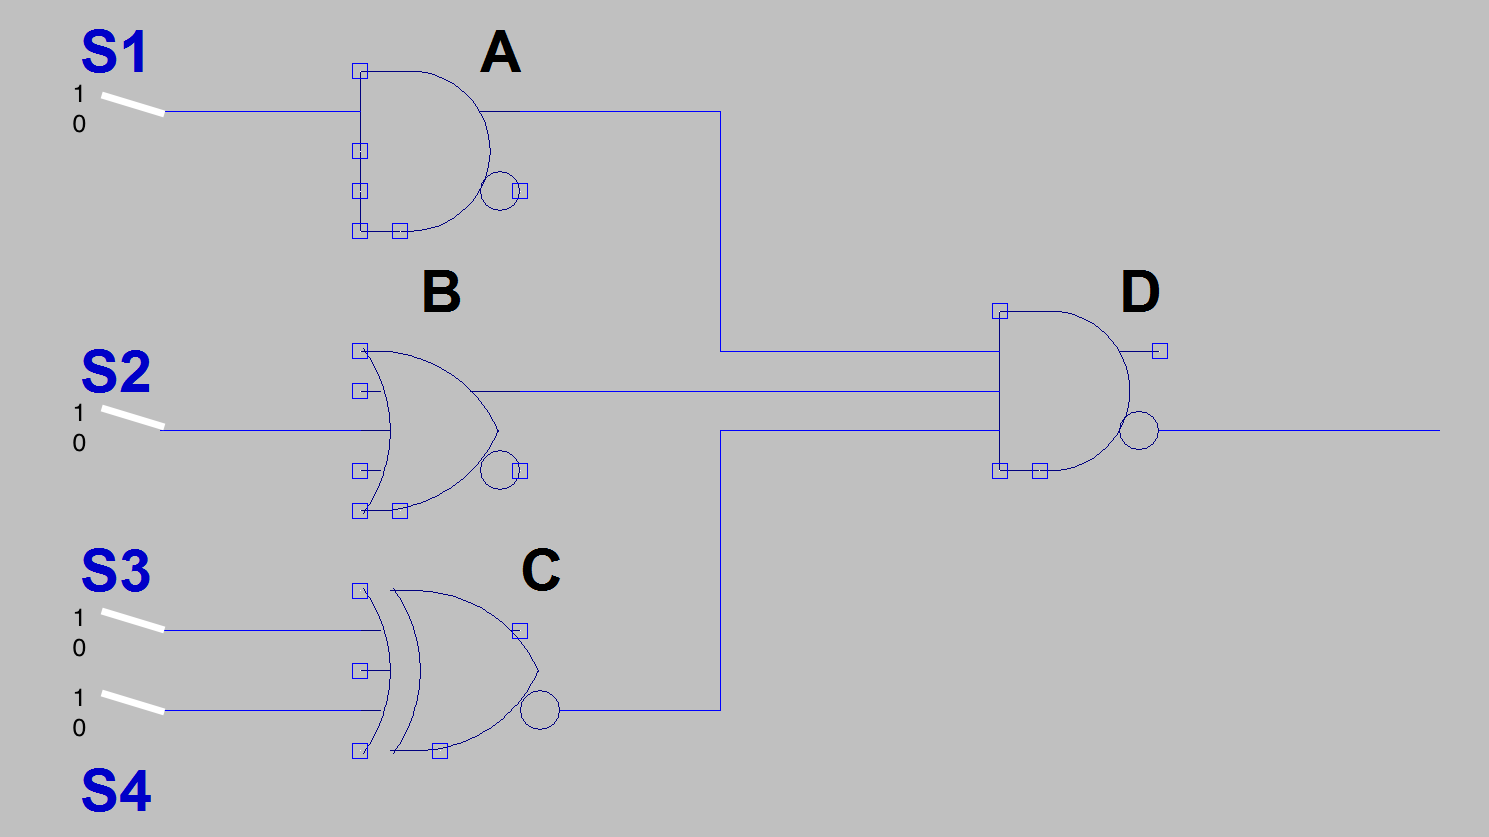
\includegraphics[width=0.8\linewidth]{circuit1.png}
  \caption{Circuit1}
  \label{fig:1}
\end{figure}
\vspace{20mm}

\n\textbf{Circuit 2 definition file.}
\begin{lstlisting}[basicstyle=\small]
DEVICES CLOCK L 100,
	SWITCH S1 1,
	SWITCH S2 0,
	SWITCH S3 0,
	DTYPE M,
	NOR A 2;
CONNECT S1 => M.SET,
	S2 => M.DATA,
	S3 => M.CLEAR,
	L  => M.CLK,
	M.Q => A.I1,
	M.QBAR => A.I2;
MONITOR A,
	QBAR;
\end{lstlisting}
\begin{figure}[H]
  \centering
  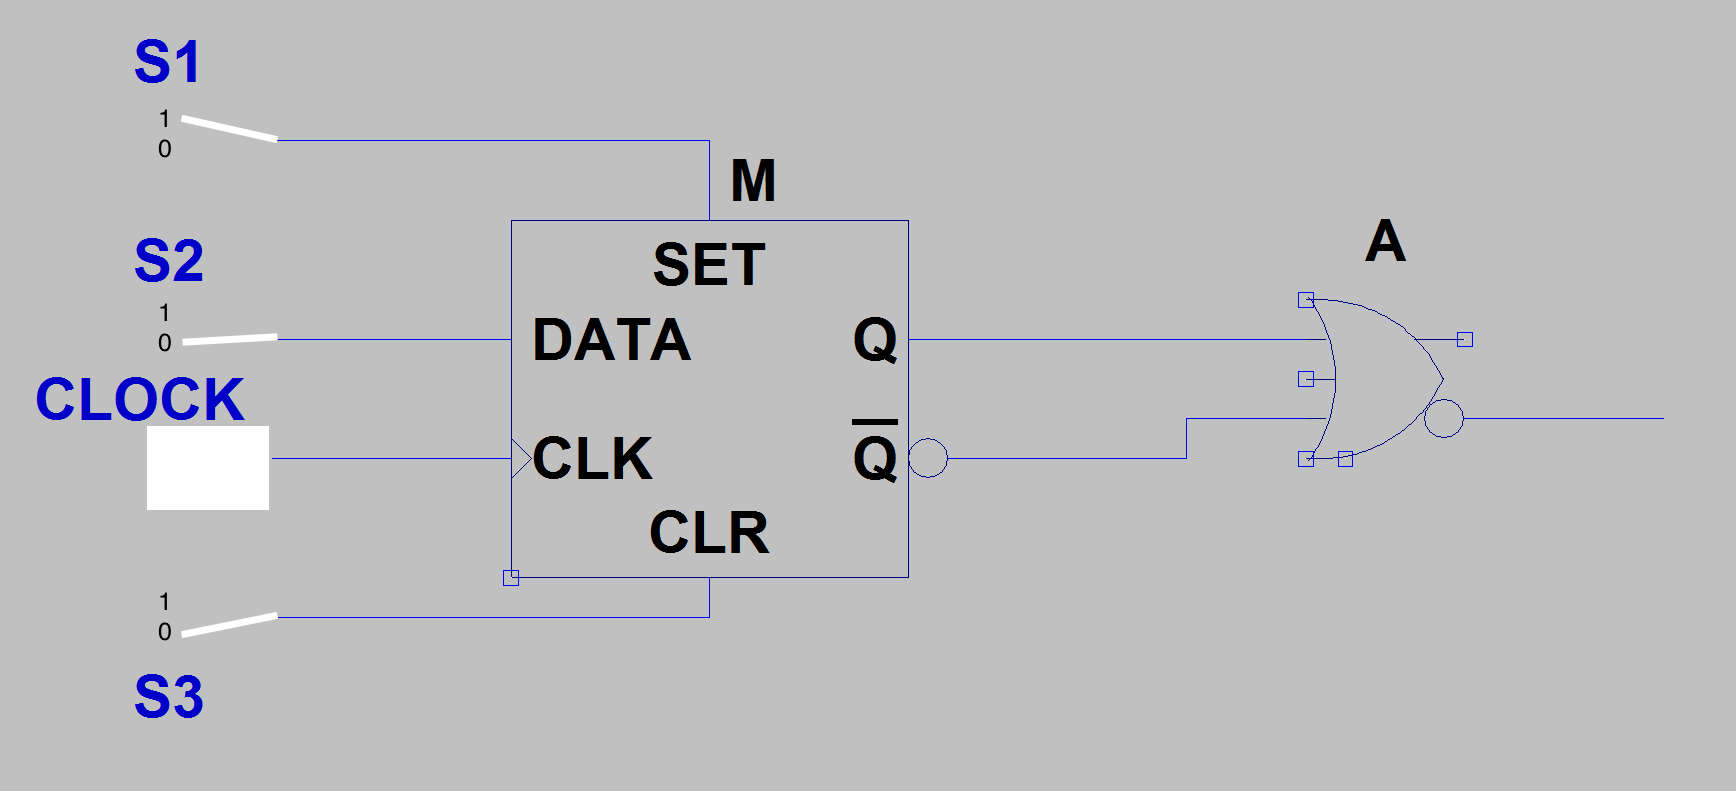
\includegraphics[width=0.8\linewidth]{circuit2.png}
  \caption{Circuit1}
  \label{fig:2}
\end{figure}

\end{document}